\documentclass{beamer}
\usepackage{apacite}
\usepackage{filecontents}
\usepackage{graphicx}
\graphicspath{ {./} }

\title{Minimum Spanning Tree Algorithms}
\subtitle{CS 375 Final Project}
\author{Tim Hung and Samuel David Bravo}
\institute{Binghamton University}
\date{May 3, 2016}

\usetheme{Copenhagen}
\setbeamertemplate{itemize items}[default]
\setbeamertemplate{enumerate items}[default]
\setbeamertemplate{navigation symbols}{}%remove navigation symbols
\setbeamertemplate{section page}
{
  \begin{centering}
    \begin{beamercolorbox}[sep=12pt,center]{part title}
      \usebeamerfont{section title}\insertsection\par
    \end{beamercolorbox}
  \end{centering}
}
\setbeamertemplate{caption}{\raggedright\insertcaption\par}

\begin{document}
\frame{\titlepage}
\section{Overview}\frame{\sectionpage}

\subsection{Minimum Spanning Trees}
\begin{frame}{Minimum Spanning Trees}
    A minimum spanning tree connects all the vertices in a graph together into
    a tree with the lightest weight possible.
\end{frame}

\subsection{Approach}
\begin{frame}{Approach}
    Algorithms:

        \begin{itemize}
        \item Kruskal's
        \item Prim's
        \end{itemize}

    Implementations:

        \begin{itemize}
        \item Adjacency List
        \item Adjacency Matrix
        \end{itemize}
\end{frame}

\subsection{Problem Statement}
\begin{frame}{Problem Statement}
    \begin{center}
    How do Prim's and Kruskal's algorithms handle graphs of different
    densities?\\
    \bigskip
    Do they depend on whether the graph is implemented as an 
    adjacency list or an adjacency matrix?
    \end{center}
\end{frame}


\section{Prim's Algorithm}\frame{\sectionpage}
\subsection{Algorithm}
\begin{frame}{Main Idea}
    \begin{center}
    Expand the tree by adding the lightest connecting edge.
    \end{center}
\end{frame}

\defverbatim[colored]\vprim {
\begin{verbatim}
EdgeContainer MST = empty
VerticesContainer keys = graph.vertices
for (v in keys) v.distance = infinity
keys[0].distance = 0

while (keys.someone_not_in_tree()) {
    Vertice v = keys.get_smallest()
    keys.add_to_tree(v)
    keys.update_distances(graph[v].neighbors)
    MST += v.edge
}
\end{verbatim}
}
\begin{frame}{Pseudocode}
\vprim
\end{frame}

\subsection{Implementation}
\begin{frame}{Key Data Structures}
    \begin{itemize}
    \item A vector of the vertices with the following information:\\
        \{weight to tree, nearest tree vertice\}
    \item A vector for holding edges included to minimum spanning tree
    \end{itemize}
\end{frame}

\begin{frame}{Functions}
    \begin{itemize}
    \item InitializeVertices, with a run time of $|V|$
    \item ExtractMin, with a run time of $lg|V|$
    \item UpdateDistances, with a run time of $|E|$
    \end{itemize}
\end{frame}

\subsection{Analysis}
\begin{frame}{Analysis of Prim's}
    \begin{itemize}
    \item Prim's is dependent on analyzing all of the nodes
    \item Extracting the minimum vertices has a running time of $|V|\lg|V|$
    \item Updating the distances has a running time of $|E|lg|V|$ 
    \item Prim's running time is of the form $O(|V|lg|V|) + O(|E|\lg|V|)$
    \item Prim's is suitable for dealing with dense graphs.
    \end{itemize}
\end{frame}


\section{Kruskal's Algorithm}\frame{\sectionpage}
\subsection{Algorithm}
\begin{frame}{Main Idea}
    \begin{itemize}
    \item Separate vertices into disjoint sets
    \item Reorder all edges by smallest weight first
    \item Loop through edges, add it to tree if its vertices are disjoint
    \end{itemize}
\end{frame}


\defverbatim[colored]\vkruskal {
\begin{verbatim}
EdgeContainer all_edges = graph.sorted_edges()

VerticesSet set = disjoint_set(v.size)
EdgeContainer MST = empty

for (Edge e : all_edges)
    v1 = e.source;
    v2 = e.destination
    if (set.are_vertices_disjoint(v1,v2))
        MST += e;
        set.join(v1,v2)
\end{verbatim}
}
\begin{frame}{Pseudocode}
\vkruskal
\end{frame}

\subsection{Implementation}
\begin{frame}{Key Data Structures}
    \begin{itemize}
    \item A vector of all the sorted edges
    \item A vector for holding edges included to minimum spanning tree
    \item A vector representing disjoint sets
    \end{itemize}
\end{frame}

\begin{frame}{Functions}
    \begin{itemize}
    \item ReadFromAdjacencyList or ReadFromAdjacencyMatrix
    \item SortEdgesSmallestFirst has a running time of $|E|\lg||E|$
    \item CreateDisjointSets has a running time of $|V|$
    \item JoinSets has a running time of $|V|$
    \item AreSetsDisjoint has a running time of $O(1)$
    \end{itemize}
\end{frame}

\subsection{Analysis}
\begin{frame}{Analysis of Kruskal's}
    \begin{itemize}
    \item Only uses graph representation for retrieving edges
    \item Sorting the edges has a running time of $|E|\lg|E|$
    \item Meanwhile, looping through edges has a running time of $|E|$
    \item The time complexity is carried by the sort, $|E|\lg|E|$
    \item Kruskal's works well with sparse graphs
    \end{itemize}   
\end{frame}


\section{Results}\frame{\sectionpage}
\subsection{Results}
\begin{frame}{Data and Results}
    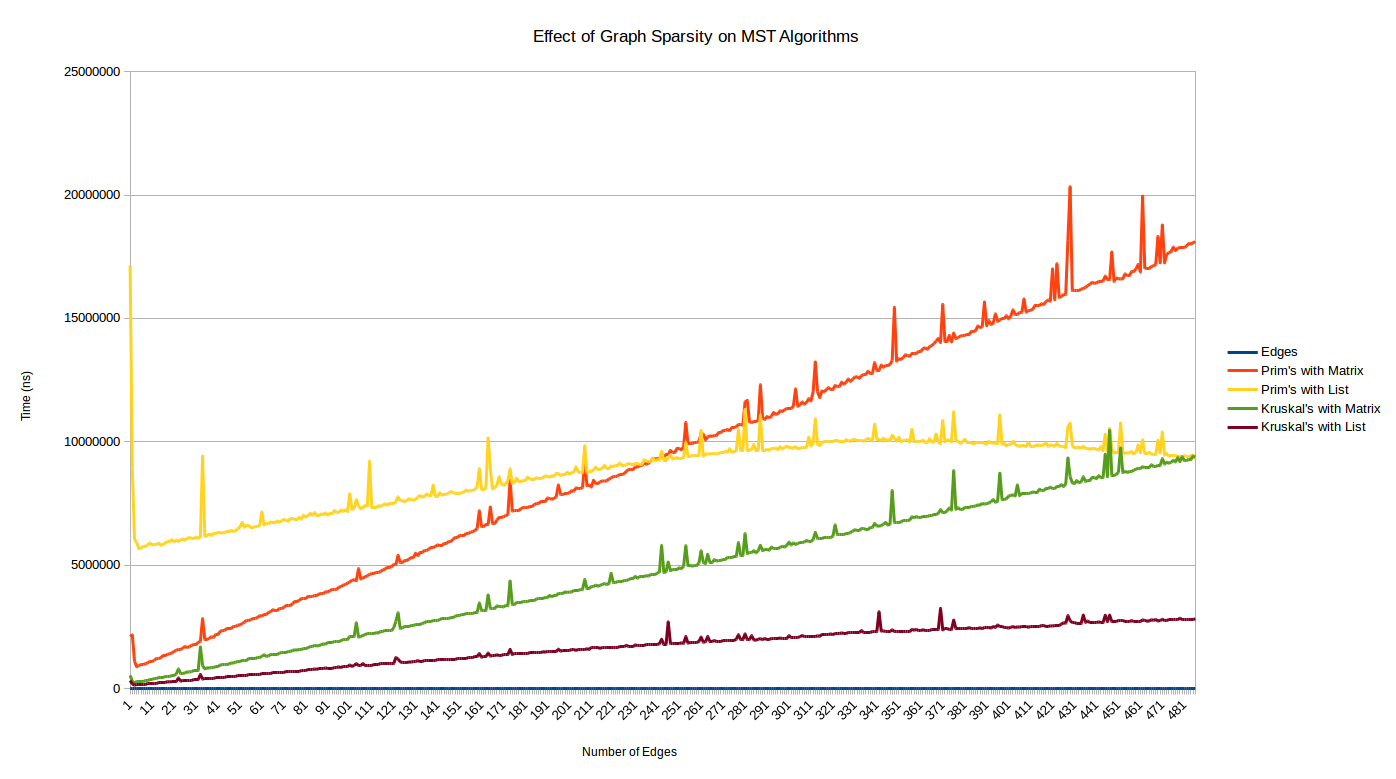
\includegraphics[width=\textwidth]{widegraph}
\end{frame}

\subsection{Limitations}
\begin{frame}{Limitations and Future Work}
    What limitations does your project currently exhibit? If you had another
    month, what could you improve? What additional tests would you run?

    \begin{itemize}
    \item Kruskal's can finish early by checking if there is only 1 set. If
    that's the case, the for loop will finish in $|V|$ instead of $|E|$.
    \end{itemize}
\end{frame}

\subsection{Questions}
\begin{frame}{Questions}
    \begin{center}
    Thank you.\\
    Any questions?
    \end{center}
\end{frame}

\end{document}
\grid
